\section{Motivation}

% ════════════════════════════════════════════════════════════════
% INTRODUCTION TO CONTRACTION THEORY
% ════════════════════════════════════════════════════════════════
\subsection{Introduction to Contraction Theory}

\begin{frame}{\insertsubsectionhead}{}

  \textbf{Contraction Theory} is a powerful tool for analyzing the stability of nonlinear systems by examining \cblue{differential dynamics}, providing insights into the behavior of \cblue{trajectories} (not points) and their convergence properties \paperinfo{ W. Lohmiller and J.-J. E. Slotine, “On contraction analysis for non-linear systems,” Automatica, 1998}.

  \begin{equation} \label{eq:pre:sys}
    \ddtt\mv{x}
    =
    \mv{f}(\mv{x},t)
    \quad
    \rightarrow
    \quad
    \text{diff. dyn. }
    \ddtt{\delta\mv{x}}
    =
    \pptfrac{\mv{f}}{\mv{x}} \delta\mv{x}
    .
  \end{equation}

  \onslide<2->
  {
  Typically used Lyapunov function is defined in terms of $\delta\mv{x}$ rather than $\mv{x}$, as follows:
  \begin{equation}
    V = \mv{x}^\top \mv{P} \mv{x}
    \quad
    \rightarrow
    \quad
    V = \delta\mv{x}^\top \mv{M}(\mv{x},t) \delta\mv{x}
    .
  \end{equation}
  }

  \onslide<3->
  {
  \begin{figure}
    \centering
    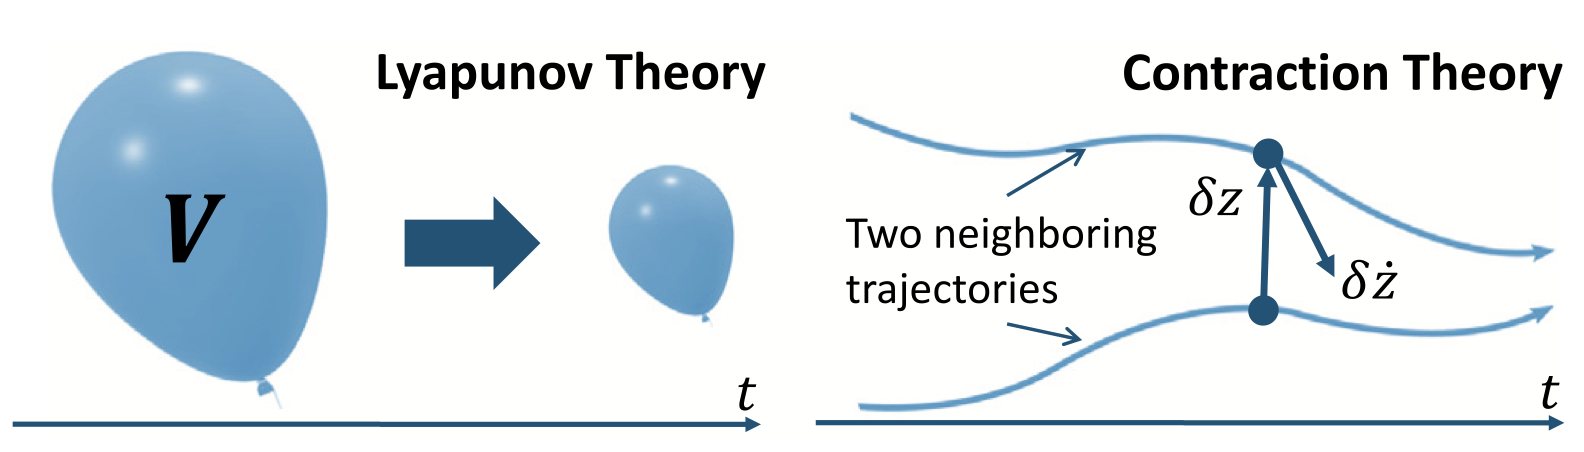
\includegraphics[width=.4\linewidth]{figures/contraction.png}
    \caption{Lyapunov theory versus contraction theory \paperinfo{H.~Tsukamoto, S.-J. Chung, and J.-J.~E. Slotine, ``Contraction theory for nonlinear stability analysis and learning-based control: A tutorial overview,'' \emph{Annual Reviews in Control}, 2021}.}
    \label{fig:contraction:theory}
  \end{figure}
  }

\end{frame}

% ————————————————————————————————————————————————————————————————
\begin{frame}{\insertsubsectionhead}{}

  Therefore, in control design, \textbf{Contraction Theory} provides:
  \begin{itemize}
    \item <2-> \textbf{Exponential Convergence}: Trajectories globally exponentially converge \cblue{regardless of initial conditions}.
    \item <3-> \textbf{Control Design}: Owing to nature of differential dynamics, \cblue{LPV control design} methods can be applied.
    \item <4-> \textbf{Stability Analysis}: The stability analysis can be simplified.
  \end{itemize}

  \vspace{1em}

  \onslide<5->
  {
  Now, the question is how to use the contraction theory in control design?
  \begin{enumerate}
    \item \textbf{Stability Analysis Tools}: Stability under a given controller can be analyzed using contraction theory.
    \item \textbf{Control Design Tools} (what we focus on): contraction theory can be used to design stabilizing controllers, \eg CCM, CV-STEM, etc. 
  \end{enumerate}
  }

\end{frame}

% ════════════════════════════════════════════════════════════════
% EXISTING APPROACHES
% ════════════════════════════════════════════════════════════════
\subsection{Existing Approaches}

\begin{frame}{\insertsubsectionhead}{Control Contraction Metric (CCM)}

  \textbf{Control Contraction Metric (CCM)} \paperinfo{I. R. Manchester and J.-J. E. Slotine, “Control contraction metrics: Convex and intrinsic criteria for nonlinear feedback design,” IEEE TAC, 2017}
  % provides a framework for designing stabilizing controllers .

  Consider a control-affine system and Lyapunov function candidate as follows:
  \begin{equation}    
    \ddtt\mv{x}
    =
    \mv{f}(\mv{x},t) + \mv{B}(\mv{x},t)\mv{u}
    \ 
    \rightarrow
    \ 
    \text{diff. dyn. }
    \ddtt{\delta\mv{x}}
    =
    \pptfrac{\mv{f}}{\mv{x}} \delta\mv{x} + \pptfrac{\mv{B}}{\mv{x}} \delta\mv{x} + \mv{B}\delta\mv{u}
    ,
    \text{ and }
    V = \delta\mv{x}^\top \mv{M}(\mv{x},t) \delta\mv{x}
    ,
  \end{equation}

  \begin{theorem}[Control Contraction Metric (CCM), informal]
    For a given system, if there exists a bounded metric $\mm{M}(\mv{x},t)$ such that holds 
    \begin{equation}
      \ddtt\mm{M} 
      + 
      2\mysym
      \left( 
        \mm{M}\pptfrac{\mv{f}}{\mv{x}} 
      \right) 
      \le 
      -2\alpha \mm{M}
      ,
      \quad
      (
        \ddtt V \le -2\alpha V
      )
      ,
    \end{equation}
    for all $\delta\mv{x}\neq 0$ such that $\delta\mv{x}^\top \mm{M}\mv{B} = 0$, then the system is \cred{universally exponentially stabilizable} via state feedback \paperinfo{H.~Tsukamoto, \etal, ``Contraction theory for nonlinear stability analysis and learning-based control: A tutorial overview,'' \emph{Annual Reviews in Control}, 2021}.
  \end{theorem}

  \begin{columns}
    \column{0.5\textwidth}     

  By using $\mm{M}$, a feedback controller $\mv{u}$ can be established considering the closest path between the current and target states in the \cred{Riemannian space} defined by $\mm{M}$, 

  \ie path integral of  $\delta\mv{u} = k(\mv{x},\delta\mv{x}, u, t)$.

    \column{0.5\textwidth}     

  \begin{figure}
    \centering
    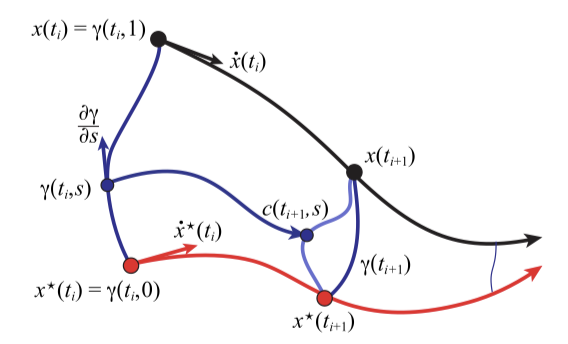
\includegraphics[width=0.49\textwidth]{figures/CCM.png}
    % \caption{Control Contraction Metric (CCM) \cite{Manchester:2017aa}.}
    \label{fig:contraction:ccm}
  \end{figure}    

  \end{columns}
\end{frame}

% ————————————————————————————————————————————————————————————————
\begin{frame}{\insertsubsectionhead}{Control Contraction Metric (CCM)}

  CMM can provide theoretical guarantees for the existence of stabilizing controllers, which can reshape the system dynamics to be contracting.

  \vspace{2em}

  However, ...
  \begin{itemize}
    \item Finding contraction metric $\mm{M}$ is \cred{computationally expensive} 
    \\
    (should be solved using SOS, LMIs, etc. using sampled data points in interested region).

    \item No consideration of input saturation and not straightforward to incorporate it.
  \end{itemize}

\end{frame}

% ————————————————————————————————————————————————————————————————
\begin{frame}{\insertsubsectionhead}{CV-STEM}

  \textbf{ConVex optimization-based Steady-state Tracking Error Minimization (CV-STEM)}\paperinfo{H. Tsukamoto, \etal, “Neural stochastic contraction metrics for learning-based
control and estimation,” IEEE Control Systems Letters, 2021}.

  \hfill

  % By defining $\delta\mv{u} = k\  \rightarrow\  \mv{u} = -\mm{K}\mm{M}(\mv{x}-\mv{x}_d)$, the contraction metric $\mm{M}$ can be obtained by solving \cred{linear matrix inequalities (LMIs)} point-wise.

  According to Theorem 2.4 in [1], by \cred{minimizing the condition number} $\chi$ of $\mm{M}$, the \cblue{steady state error} can be reduced.
  \begin{equation}
    \downarrow \chi \text{(condition number of $\mm{M}$)} \quad \rightarrow \quad \downarrow \text{steady state error}
  \end{equation}

  The control input can be simply obtained by
  \begin{equation}
      \mv{u} = \mv{u}_d - \mv{R}^{-1}\mv{B}^\top \mm{M}(\mv{x}-\mv{x}_d)
        ,\quad
        (
          \mv{M} \text{ is obtained by \cred{solving LMIs which minimizes $\chi$}.}
        )
  \end{equation}

  Main features of CV-STEM are as follows:
  \begin{itemize}
      \item Easy to implement (step-wise convex condition and affine control law).
      \item Due to the use of LMIs, it should be solved in advance.
      % \item According to the objective function, typically, $\mv{M}$ is designed to be identity matrix and $\nu$ is maximized, which results in \cred{a simple state feedback controller with a large proportional gain}.
      \item Still has no consideration of input saturation.
  \end{itemize}
\end{frame}

% ════════════════════════════════════════════════════════════════
% COMMON LIMITATIONS
% ════════════════════════════════════════════════════════════════
\subsection{Common Limitations}

\begin{frame}{\insertsubsectionhead}{}

  \textbf{What if} the control input is saturated?

  \begin{equation}
    \ddtt\mv{x} = \mv{f}(\mv{x},t) + \mv{B}(\mv{x},t)\cred{\mysat(\mv{u})}
  \end{equation}

  Typically, contraction theory-based control design methods does not consider input constraints, which can lead to \cred{undesirable behavior} in practical applications.

  Furthermore, the existing methods compute $\mm{M}$ using matrix-space optimization problems, explicitly imposing constraints in input vector space is not straightforward.
\end{frame}

% ════════════════════════════════════════════════════════════════
% SUMMARY AND MOTIVATION FOR PROPOSED METHOD
% ════════════════════════════════════════════════════════════════
\subsection{Summary and Motivation for Proposed Method}

\begin{frame}{\insertsubsectionhead}{}

  % Summary of the discussion on contraction theory-based control design methods:

  % \begin{itemize}
  %   \item CCM is a powerful tool providing the existence of stabilizing controllers.
  %   \item CV-STEM provides a more computationally efficient approach to find contraction metric $\mm{M}$ in a point-wise manner.
  %   \item However, both CCM and CV-STEM still \dots
  %   \begin{itemize}
  %     \item Computationally expensive (should be solved in advance).
  %     \item Difficult to handle constraints, such as input saturation.
  %   \end{itemize}
  % \end{itemize}

  % \hfill

  The proposed approach \dots

  \begin{itemize}
    \item Transforms the \cred{matrix-space optimization problem} for $\mm{M}$ into a \cblue{vector-space optimization problem} by \textbf{projecting the contraction condition} into a vector space.
    \item Handles the input saturation in a more direct way by \cred{incorporating the input saturation} into the optimization problem.
  \end{itemize}
    
\end{frame}


% \begin{frame}{\insertsubsectionhead}{}

%     CCM is similar to the control Lyapunov function (CLF) in that it provides a condition for the existence of a stabilizing controller.

%     \begin{itemize}
%         \item Both CCM and CLF provide conditions for the \cred{existence of stabilizing controllers}.
%         \item CCM focuses on the contraction of trajectories in a Riemannian space defined by a metric $\mm{M}$, while CLF focuses on the decrease of a scalar function $V$ along system trajectories.
%         % \item CCM can be seen as a generalization of CLF, where the contraction metric $\mm{M}$ plays a role similar to the Lyapunov function $V$ in CLF, but with a focus on the geometry of the state space rather than just scalar values.
%     \end{itemize} 

%     \hfill

%     There are several limitations as follows:

%     \begin{itemize}
%         \item Finding a solution of CCM and CLF is non-convex and \cred{computationally expensive}, (should be solved iteratively and in advance).
%         \item \cblue{Constraint handling} is not straightforward, and it is difficult to guarantee the satisfaction of constraints during the control design process.
%         \item Since CCM and CLF are designed based on global stability properties, they may be \cred{conservative}.
%     \end{itemize}
% \end{frame}